\documentclass{pssbmac}

%%%%%%%%%%%%%%%%%%%%%%%%%%%%%%%%%%%%%%%%%%%%%%%%%%%%%%%%%%%%%%%%%%%%%%%%
%% POR FAVOR, NÃO FAÇA MUDANÇAS NESSE PADRÃO QUE ACARRETEM  EM
%% ALTERAÇÃO NA FORMATAÇÃO FINAL DO TEXTO
%%%%%%%%%%%%%%%%%%%%%%%%%%%%%%%%%%%%%%%%%%%%%%%%%%%%%%%%%%%%%%%%%%%%%%%%

%%%%%%%%%%%%%%%%%%%%%%%%%%%%%%%%%%%%%%%%%%%%%%%%%%%%%%%%%%%%%%%%%%%%%%%%
% POR FAVOR, ESCOLHA CONFORME O CASO
%%%%%%%%%%%%%%%%%%%%%%%%%%%%%%%%%%%%%%%%%%%%%%%%%%%%%%%%%%%%%%%%%%%%%%%%
%\usepackage[brazil]{babel} % texto em Português
\usepackage[english]{babel} % texto em Inglês

%\usepackage[latin1]{inputenc} % acentuação em Português ISO-8859-1
\usepackage[utf8]{inputenc} % acentuação em Português UTF-8
%%%%%%%%%%%%%%%%%%%%%%%%%%%%%%%%%%%%%%%%%%%%%%%%%%%%%%%%%%%%%%%%%%%%%%%%


%%%%%%%%%%%%%%%%%%%%%%%%%%%%%%%%%%%%%%%%%%%%%%%%%%%%%%%%%%%%%%%%%%%%%%%%
%% POR FAVOR, NÃO ALTERAR
%%%%%%%%%%%%%%%%%%%%%%%%%%%%%%%%%%%%%%%%%%%%%%%%%%%%%%%%%%%%%%%%%%%%%%%%
\usepackage[T1]{fontenc}
\usepackage{float}
\usepackage{graphics}
\usepackage{graphicx}
\usepackage{epsfig}
\usepackage{indentfirst}
\usepackage{amsmath, amsfonts, amssymb, amsthm, mathtools}
\usepackage{url}
\usepackage{csquotes}
\usepackage{lipsum}
% Ambientes pré-definidos
\newtheorem{theorem}{Theorem}[section]
\newtheorem{lemma}{Lemma}[section]
\newtheorem{proposition}{Proposition}[section]
\newtheorem{definition}{Definition}[section]
\newtheorem{remark}{Remark}[section]
\newtheorem{corollary}{Corollary}[section]
\newtheorem{teorema}{Teorema}[section]
\newtheorem{lema}{Lema}[section]
\newtheorem{prop}{Proposi\c{c}\~ao}[section]
\newtheorem{defi}{Defini\c{c}\~ao}[section]
\newtheorem{obs}{Observa\c{c}\~ao}[section]
\newtheorem{cor}{Corol\'ario}[section]

% ref bibliográficas
\usepackage[backend=biber, style=numeric-comp, maxnames=50]{biblatex}
\addbibresource{../refs.bib}
\DeclareTextFontCommand{\emph}{\boldmath\bfseries}
\DefineBibliographyStrings{brazil}{phdthesis = {Tese de doutorado}}
\DefineBibliographyStrings{brazil}{mathesis = {Disserta\c{c}\~{a}o de mestrado}}
\DefineBibliographyStrings{english}{mathesis = {Master dissertation}}
%%%%%%%%%%%%%%%%%%%%%%%%%%%%%%%%%%%%%%%%%%%%%%%%%%%%%%%%%%%%%%%%%%%%%%%%


\begin{document}

%%%%%%%%%%%%%%%%%%%%%%%%%%%%%%%%%%%%%%%%%%%%%%%%%%%%%%%%%%%%%%%%%%%%%%%%
% TÍTULO E AUTORAS(ES)
%%%%%%%%%%%%%%%%%%%%%%%%%%%%%%%%%%%%%%%%%%%%%%%%%%%%%%%%%%%%%%%%%%%%%%%%

\title{Vulnerability of urban road networks to floods - A case study in São Paulo, Brazil}

\author{
    {\large Pedro Augusto Borges dos Santos}\thanks{pedro.borges@inpe.br},\  {\large Dr. Leonardo Bacelar Lima Santos}\thanks{leonardo.bacelar@inpe.br}\\
    {\small Instituto Nacional de Pesquisas Espaciais, São José dos Campos, SP}
}
\criartitulo
%%%%%%%%%%%%%%%%%%%%%%%%%%%%%%%%%%%%%%%%%%%%%%%%%%%%%%%%%%%%%%%%%%%%%%%%


%%%%%%%%%%%%%%%%%%%%%%%%%%%%%%%%%%%%%%%%%%%%%%%%%%%%%%%%%%%%%%%%%%%%%%%%
% TEXTO
%%%%%%%%%%%%%%%%%%%%%%%%%%%%%%%%%%%%%%%%%%%%%%%%%%%%%%%%%%%%%%%%%%%%%%%%

\begin{abstract}

\lipsum[1]

\noindent
{\bf Keywords}.
\end{abstract}

\section{Introduction}

Road networks are vulnerable to natural disasters, such as floods, which can cause damage to infrastructure and adversely affect travel and/or local populations on degraded networks. Studying and analyzing the vulnerability of road networks helps prioritize planning, budgeting, and maintenance, as well as prepare effective emergency response plans \cite{balijepalliMeasuringVulnerabilityRoad2014}. Each city has its own characteristics of road design, intersection density, mobility patterns, and population distribution, which can directly influence results.

% Although the literature on road network vulnerability has advanced in proposing metrics and methodologies, it is still important to investigate and understand how flooding events impact different parts of the network based on their vulnerability. Each city has its own characteristics of road design, intersection density, mobility patterns, and population distribution, which can directly influence results.

In this scenario, the objective of this study is to assess the vulnerability of urban road networks based on topology and the occurrence of floods. Using areas of the city of São Paulo, Brazil, as a case study, this manuscript explores the relationship between topological properties, flood occurrence, and population distribution in the studied area. For this work, vulnerability is defined as the degree to which a road network is susceptible to performance degradation when exposed to adverse events.

Previous studies have also investigated the vulnerability of transport and road networks using graph-based approaches and the analysis of flood occurrence. Regarding road network topology, previous studies have focused on vulnerability in urban road networks \cite{morelliMeasuringUrbanRoad2021} and rural road networks \cite{santosVulnerabilityAnalysisComplex2023}, analyzing vulnerability to flooding in mobility systems.

% This manuscript is organized as follows: Section 2 describes the study area, data, and methods used in this research. Section 3 presents the results of the analysis. Section 4 discusses the findings and provides insights into the implications of the research, concludes the manuscript, and suggests future research directions.


\section{Material and methods}

\subsection{Study area}

The area investigated included five parts of the Tamanduateí (TTI) river basin entirely inside the city of São Paulo\cite{prefeituradesaopauloPlanoDiretorDrenagem2024}. The road network was selected based on origin/destination (OD) zones from the city of São Paulo, which intersected the selected parts of the basin. These OD zones were developed to count and manage traffic in the city \cite{metrospPesquisaOrigemDestino2023}. In total, 92 OD zones were considered (from a total of 527). From the selected OD zones, it was possible to load the road network graph from November 2025. The flood occurrence locations were loaded as point objects \cite{cge-spAlagamentos2025}, between 2022-01 and 2025-04, and were associated to the nearest edge object in the graph.

% \begin{figure}[H]
% \centering
% 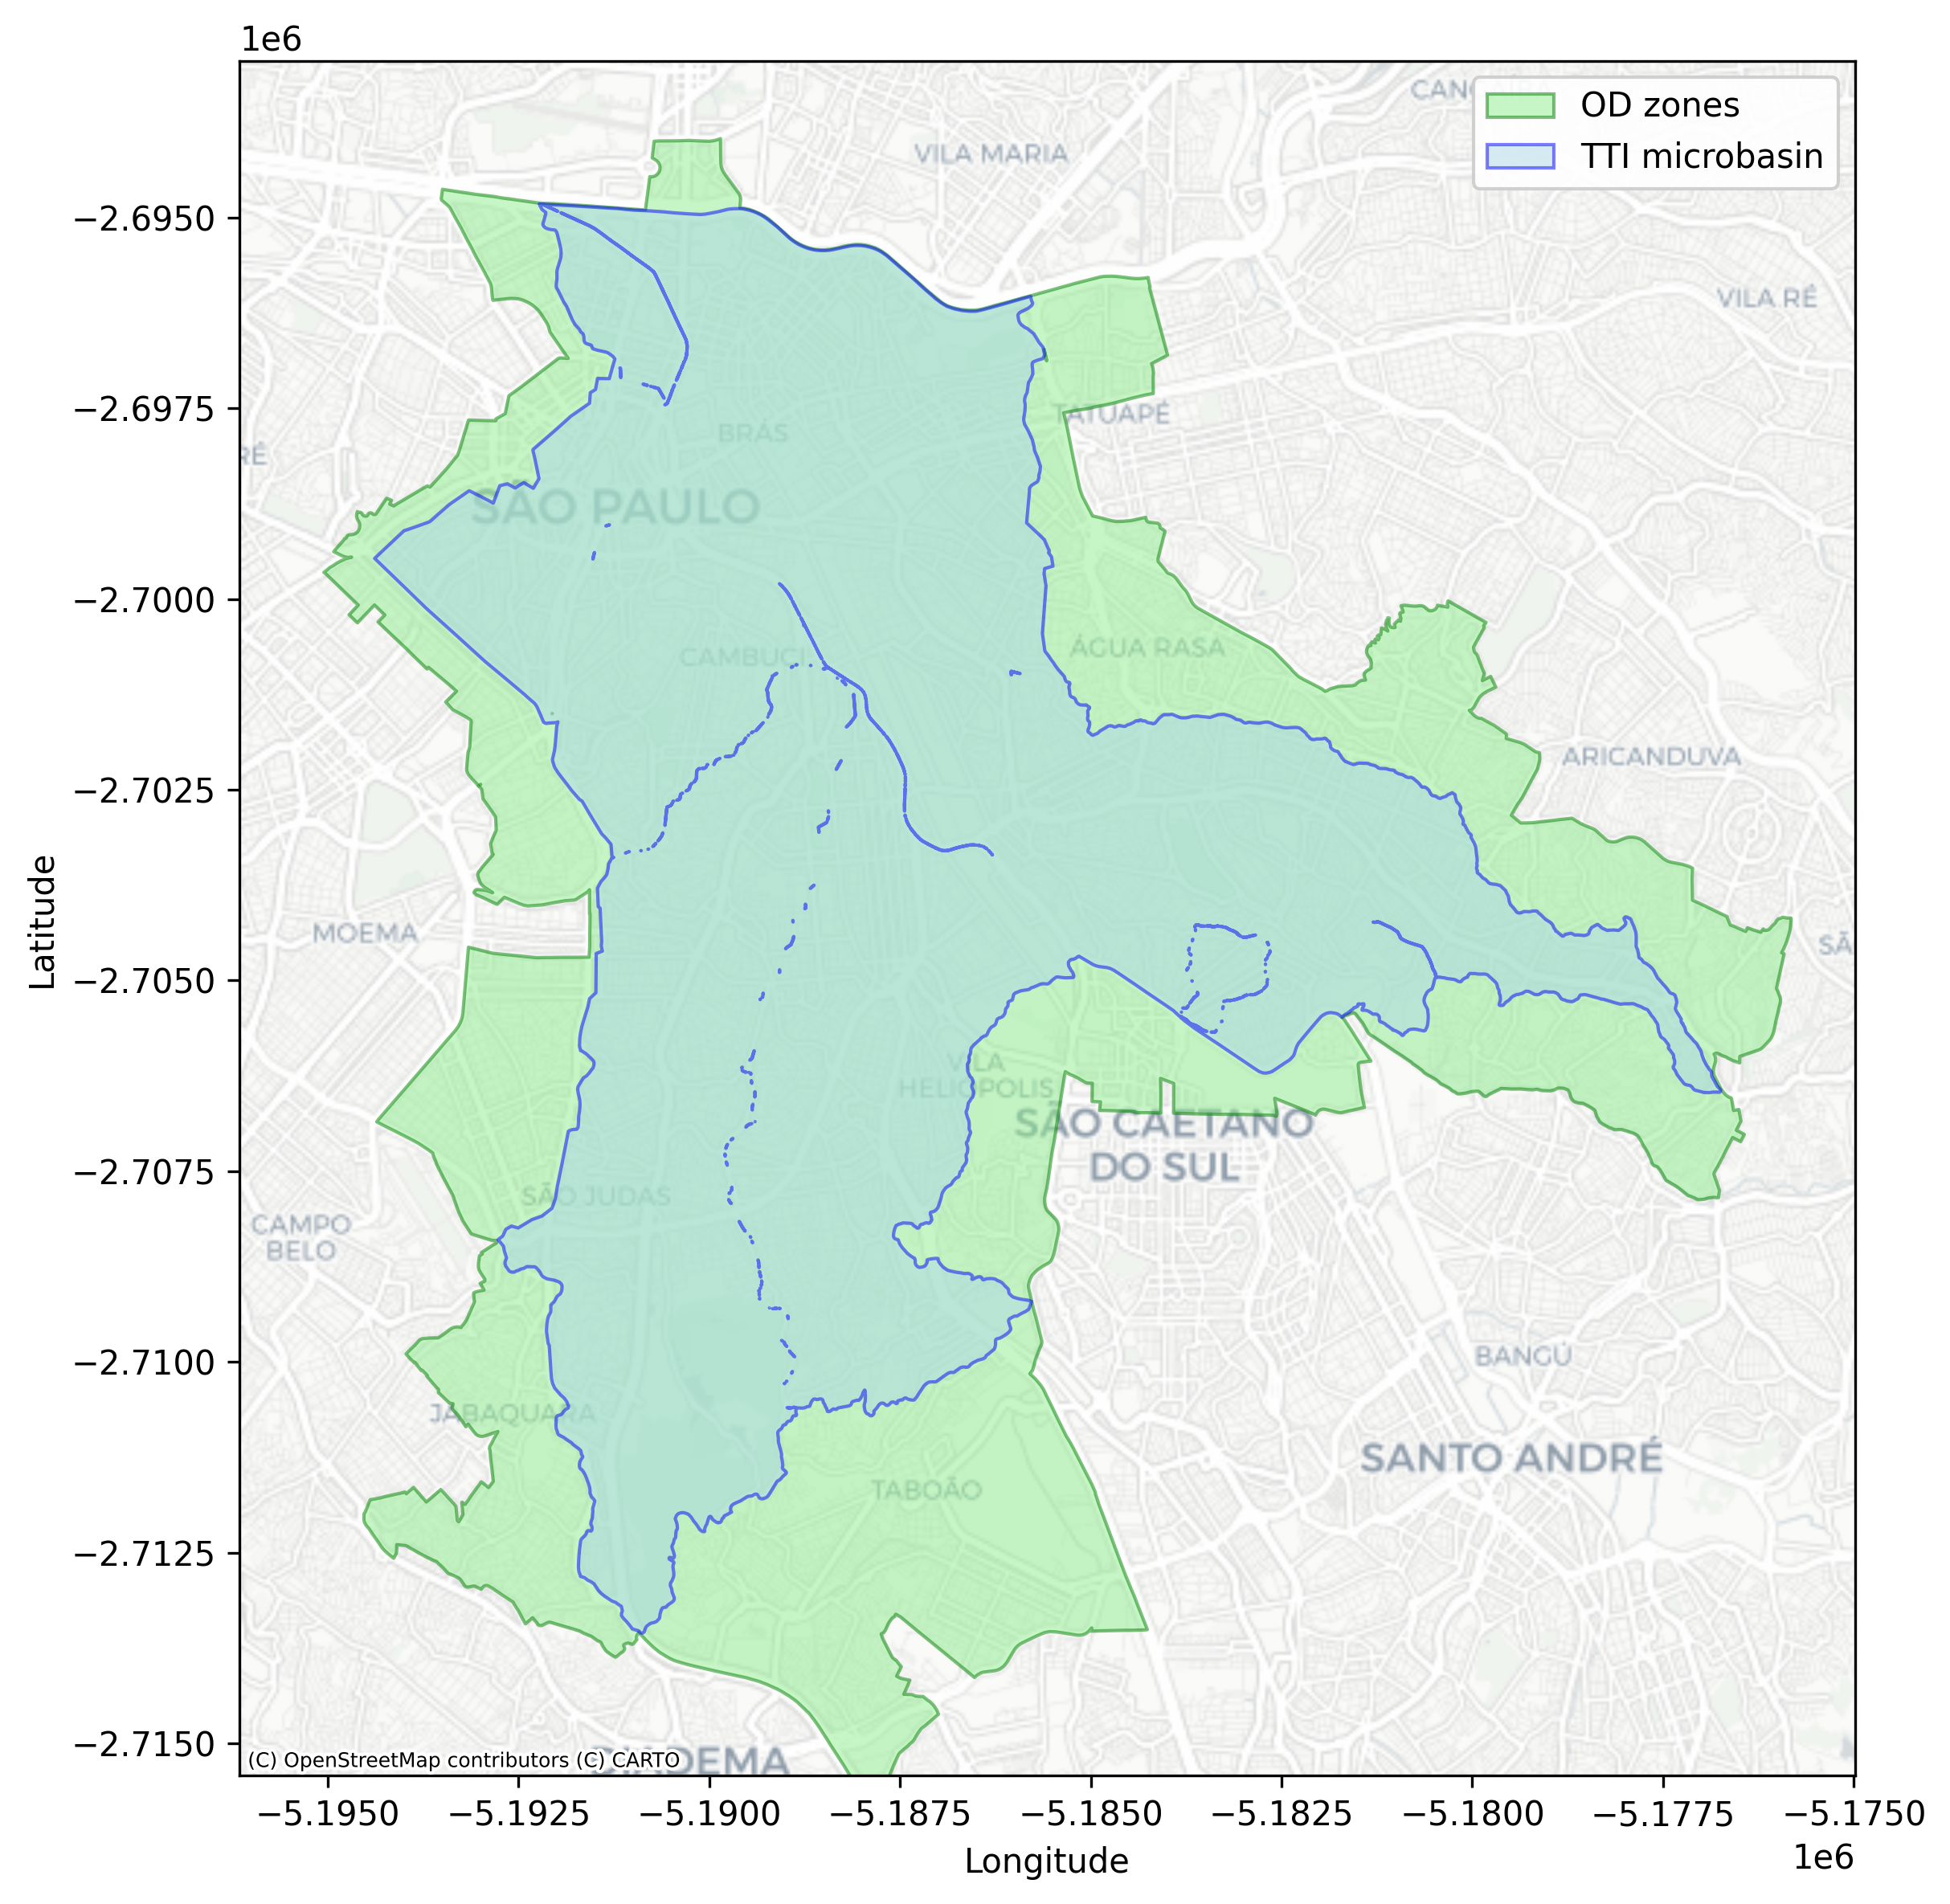
\includegraphics[width=0.75\textwidth]{../plot/study_area_map.png}
% \caption{Study scenario}
% \label{fig:area}
% \end{figure}

% From the selected OD zones, it was possible to load the road network graph from November 2025. The flood occurrence locations were loaded as point objects \cite{cge-spAlagamentos2025}, between 2022-01 and 2025-04, and were associated to the nearest edge object in the graph. Figure \ref{fig:flood} presents the loaded road network and flood locations.

% \begin{figure}[H]
% \centering
% 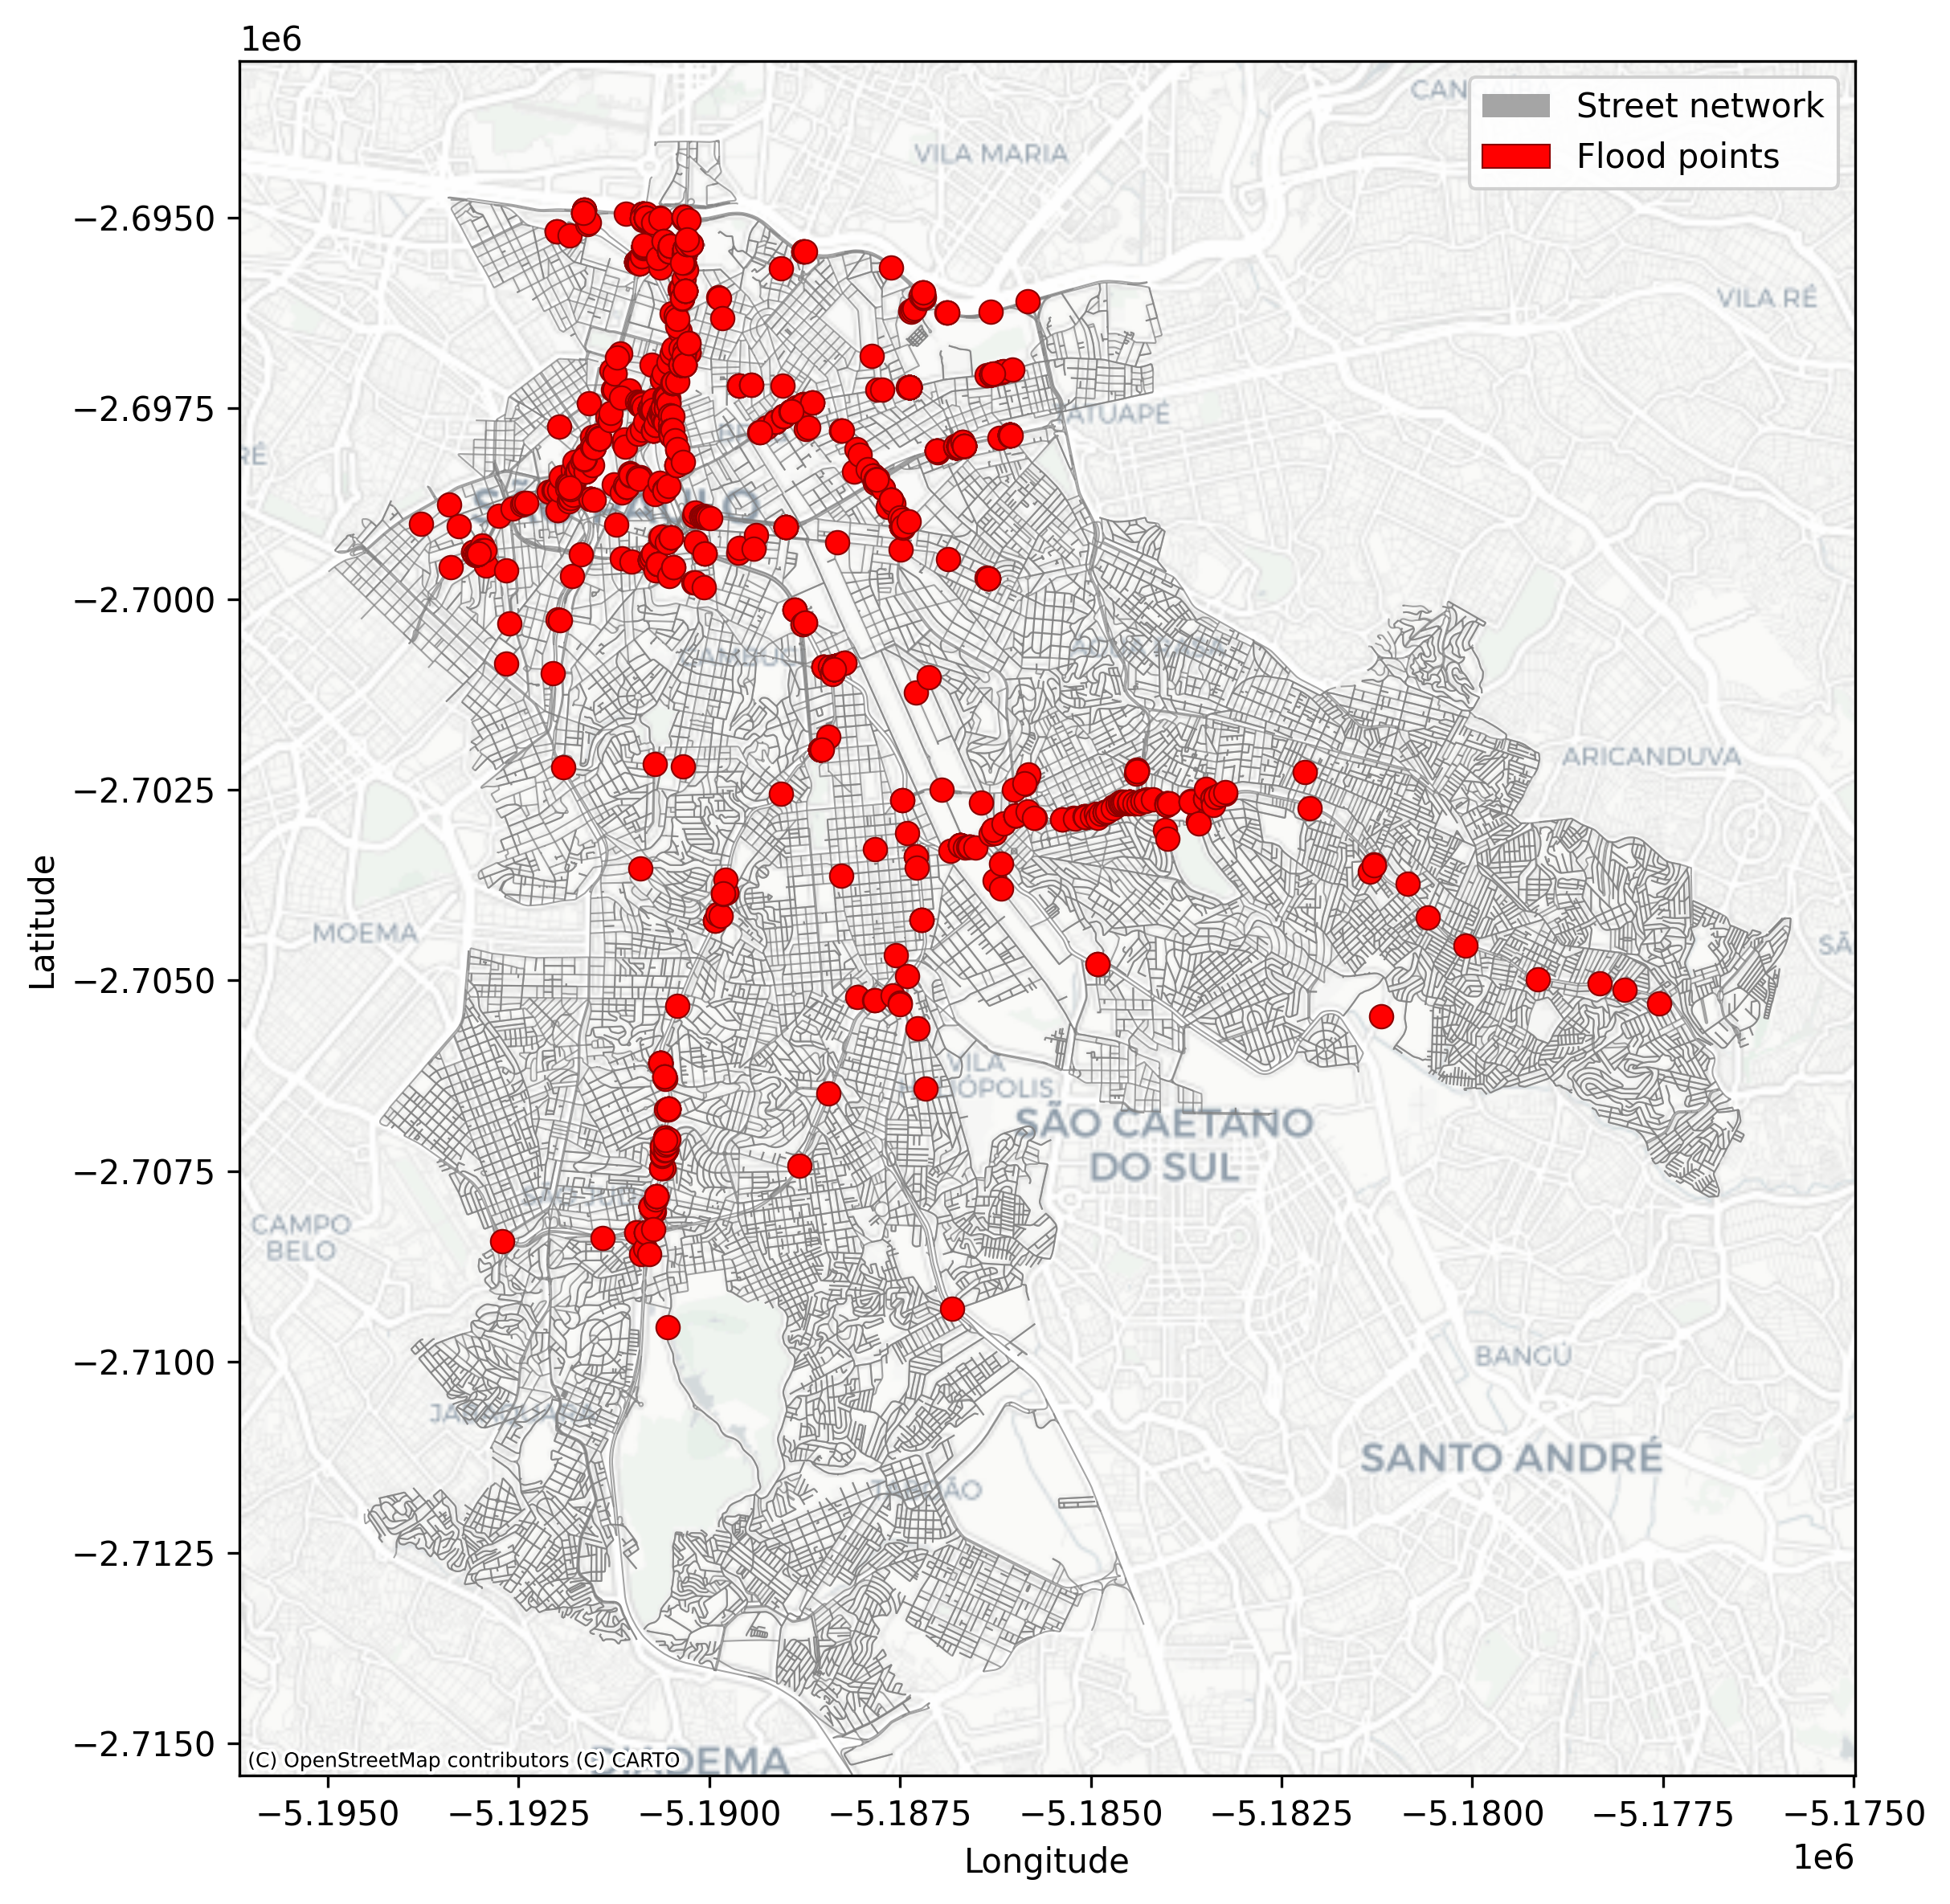
\includegraphics[width=.6\textwidth]{../plot/network_flood_map.png}
% \caption{Road network and flood points}
% \label{fig:flood}
% \end{figure}

\subsection{Graph analysis}

The road network presented in this work is represented by a graph $G$, where each intersection is a node and each road segment is an edge, therefore,  $V$ is a set of vertices (or nodes) and $E$ is a set of edges (or links) that connects pairs of nodes (or connects a node to itself): $G = (V, E)$. The edge ($e$) betweenness centrality ($c_B(e)$) is calculated by the sum of the fraction of all-pairs shortest paths that pass through that edge, as the following Equation shows:

\begin{equation}
c_B(e) = \sum_{s, t \in V} \frac{\sigma(s, t | e)}{\sigma(s, t)}; \label{eq:ebc}
\end{equation}

where $V$ is the set of nodes, $\sigma(s, t)$ is the number of shortest $(s, t)$-paths, and $\sigma(s, t | e)$ is the number of those paths passing through edge $e$ \cite{costaCharacterizationComplexNetworks2007}.

Also, the node degree ($k_i$) was calculated, which is the number of edges connected to that node. This is known as adjacency ($a_{i j}$). When two nodes $i$ and $j$ are said to be neighbors, then $a_{i j} \neq 0$. The following Equation \ref{eq:ki} shows the computation of $k_i$ \cite{costaCharacterizationComplexNetworks2007}:

\begin{equation}
k_i = \sum_j a_{i j} \label{eq:ki}
\end{equation}

% Regarding vulnerability, the edge betweenness centrality (EBC) of the road network was compared to the flood count for each edge. The count of flood events for each edge was calculated using a nearest spatial join approach, where the nearest edge to each flood point was considered.

\subsection{Population data}

The population data was collected from the Brazilian Demographic Census of 2022 \cite{ibgeCensoDemografico20222022}. The available data is aggregated by census tracts, and only the ones inside the study area were selected, by intersection to the OD zones. After selecting the census tracts, two steps were necessary to migrate population data from tracts to the network edges. First, a spatial join between tracts and nodes was performed. The population was equally divided among each node $i$ within the same census tract. Then, for each edge $e$ between nodes $(u, v)$, the population ($P_e(u, v)$) was calculated as the sum of the population of node $u$ ($P_u$) divided by its degree ($k_u$) plus the population of node $v$ ($P_v$) divided by its degree ($k_v$)

\begin{equation}
P_e(u, v) = \frac{P_u}{k_u} + \frac{P_v}{k_v} \label{eq:pop}
\end{equation}

% \subsection{Computational tools}

% The analysis and most computational methods were performed using the Python programming language, version 3.12.12. The following packages were mainly used: \verb|osmnx| \cite{boeingModelingAnalyzingUrban2025}, \verb|networkx| \cite{hagbergExploringNetworkStructure2008}, and \verb|geopandas| \cite{jorisvandenbosscheGeopandasGeopandasV1112025}. The code was packaged and is available in the following repository: \textcite{santosTamaproject2025}.

\section{Results}

The loaded road network graph has 21,045 nodes and 48,769 edges. Figure \ref{fig:power} shows the probability of node degree per degree value. There is a high probability of degree values between 2 and 6. The values vary between 1 and 10. The network does not strictly follow a power-law behavior.

\begin{figure}[H]
\centering
\includegraphics[width=.7\textwidth]{../plot/degree_distribution.png}
\caption{Node degree distribution}
\label{fig:power}
\end{figure}

The map in Figure \ref{fig:ebcmap} shows the EBC of the road network. Most road sections have low EBC values (zero or near zero). Only a few road sections have higher EBC values, indicating that they are more vulnerable to events that impact serviceability.

\begin{figure}[htbp]
\centering
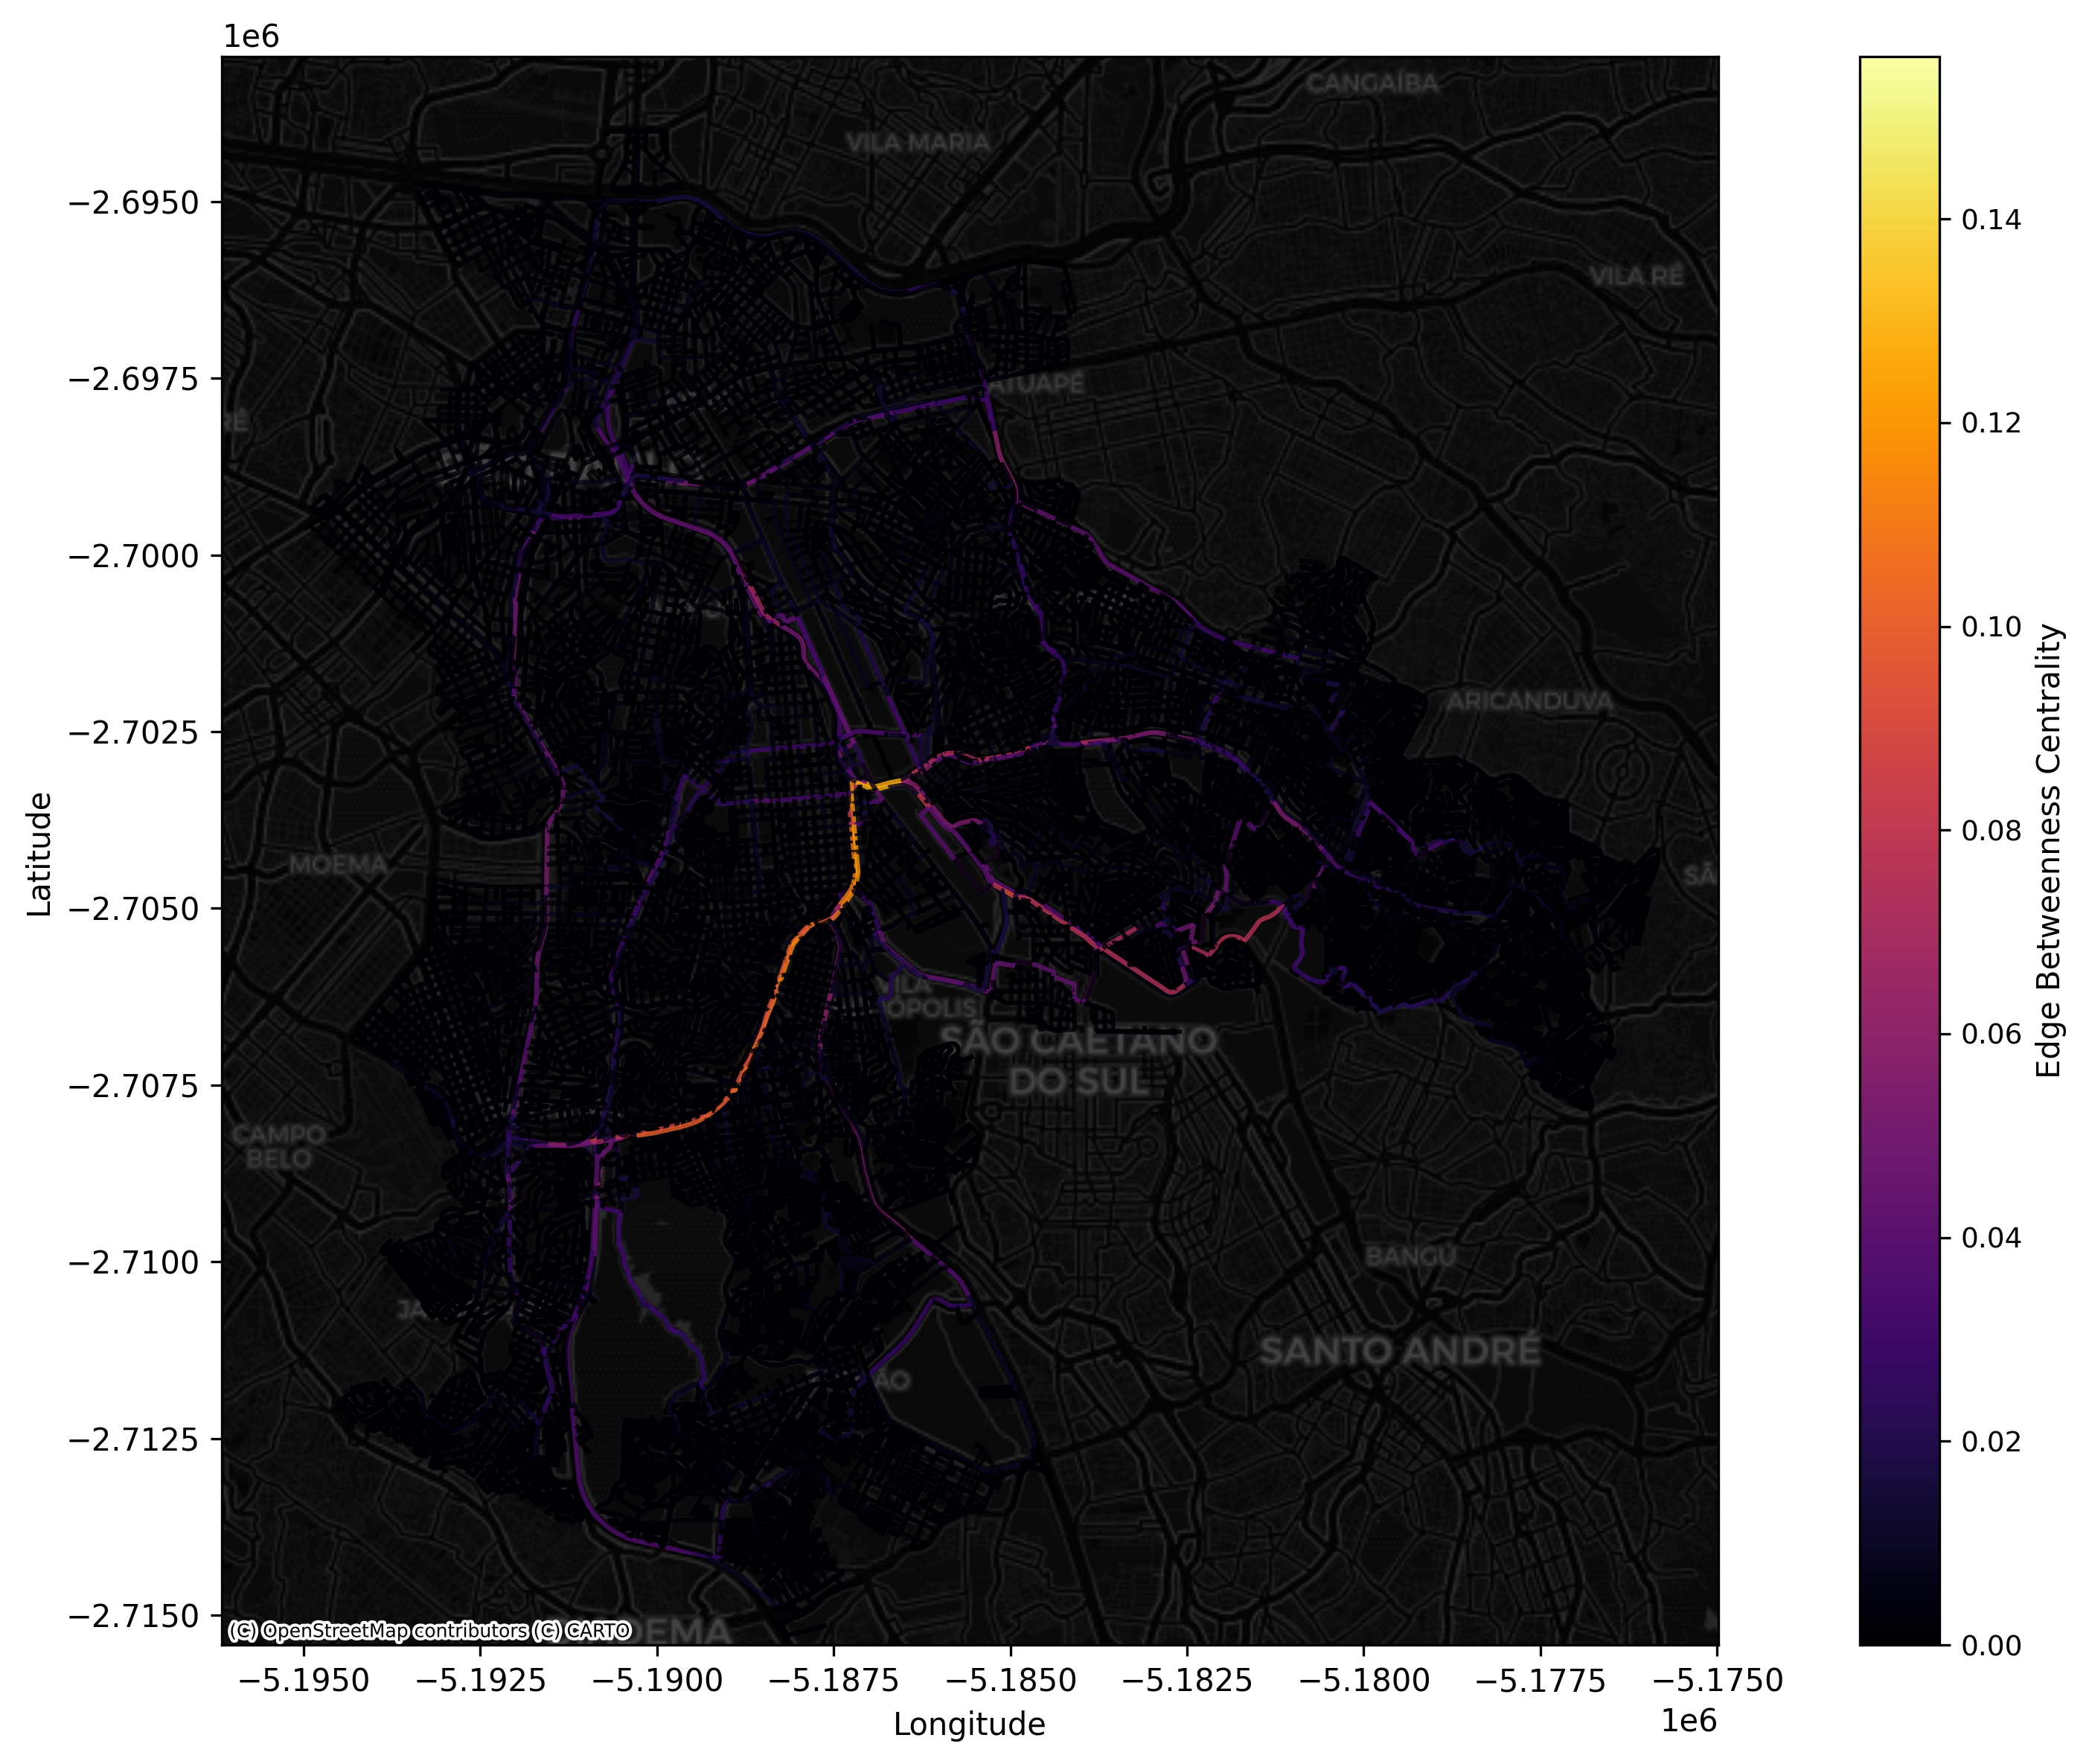
\includegraphics[width=.7\textwidth]{../plot/network_ebc_map.png}
\caption{Network EBC results}
\label{fig:ebcmap}
\end{figure}

% \begin{figure}[H]
% \centering
% \includegraphics[width=.8\textwidth]{../plot/population_map.png}
% \caption{Population per census tract}
% \label{fig:popcensus}
% \end{figure}

A total of 7,329 census tracts were loaded and selected. The map in Figure \ref{fig:popedge} presents the estimated population for all 48,769 graph edges, with a total population of 2,137,552. Approximately 95\% of the edges have population values below 100.

\begin{figure}[htbp]
\centering
\includegraphics[width=.7\textwidth]{../plot/edges_population_map.png}
\caption{Population per network edge}
\label{fig:popedge}
\end{figure}

Figure \ref{fig:ebc-flood-scatter} shows the normalized flood count, which is the flood value divided by the total count of edges in each range of EBC values (bin size of 0.01), per EBC value. Edges in the ranges of 0.06-0.07 and 0.12-0.13 show the highest values of normalized flood count, which indicates parts of the road network that are considerably more vulnerable compared to other parts of the network.

\begin{figure}[H]
\centering
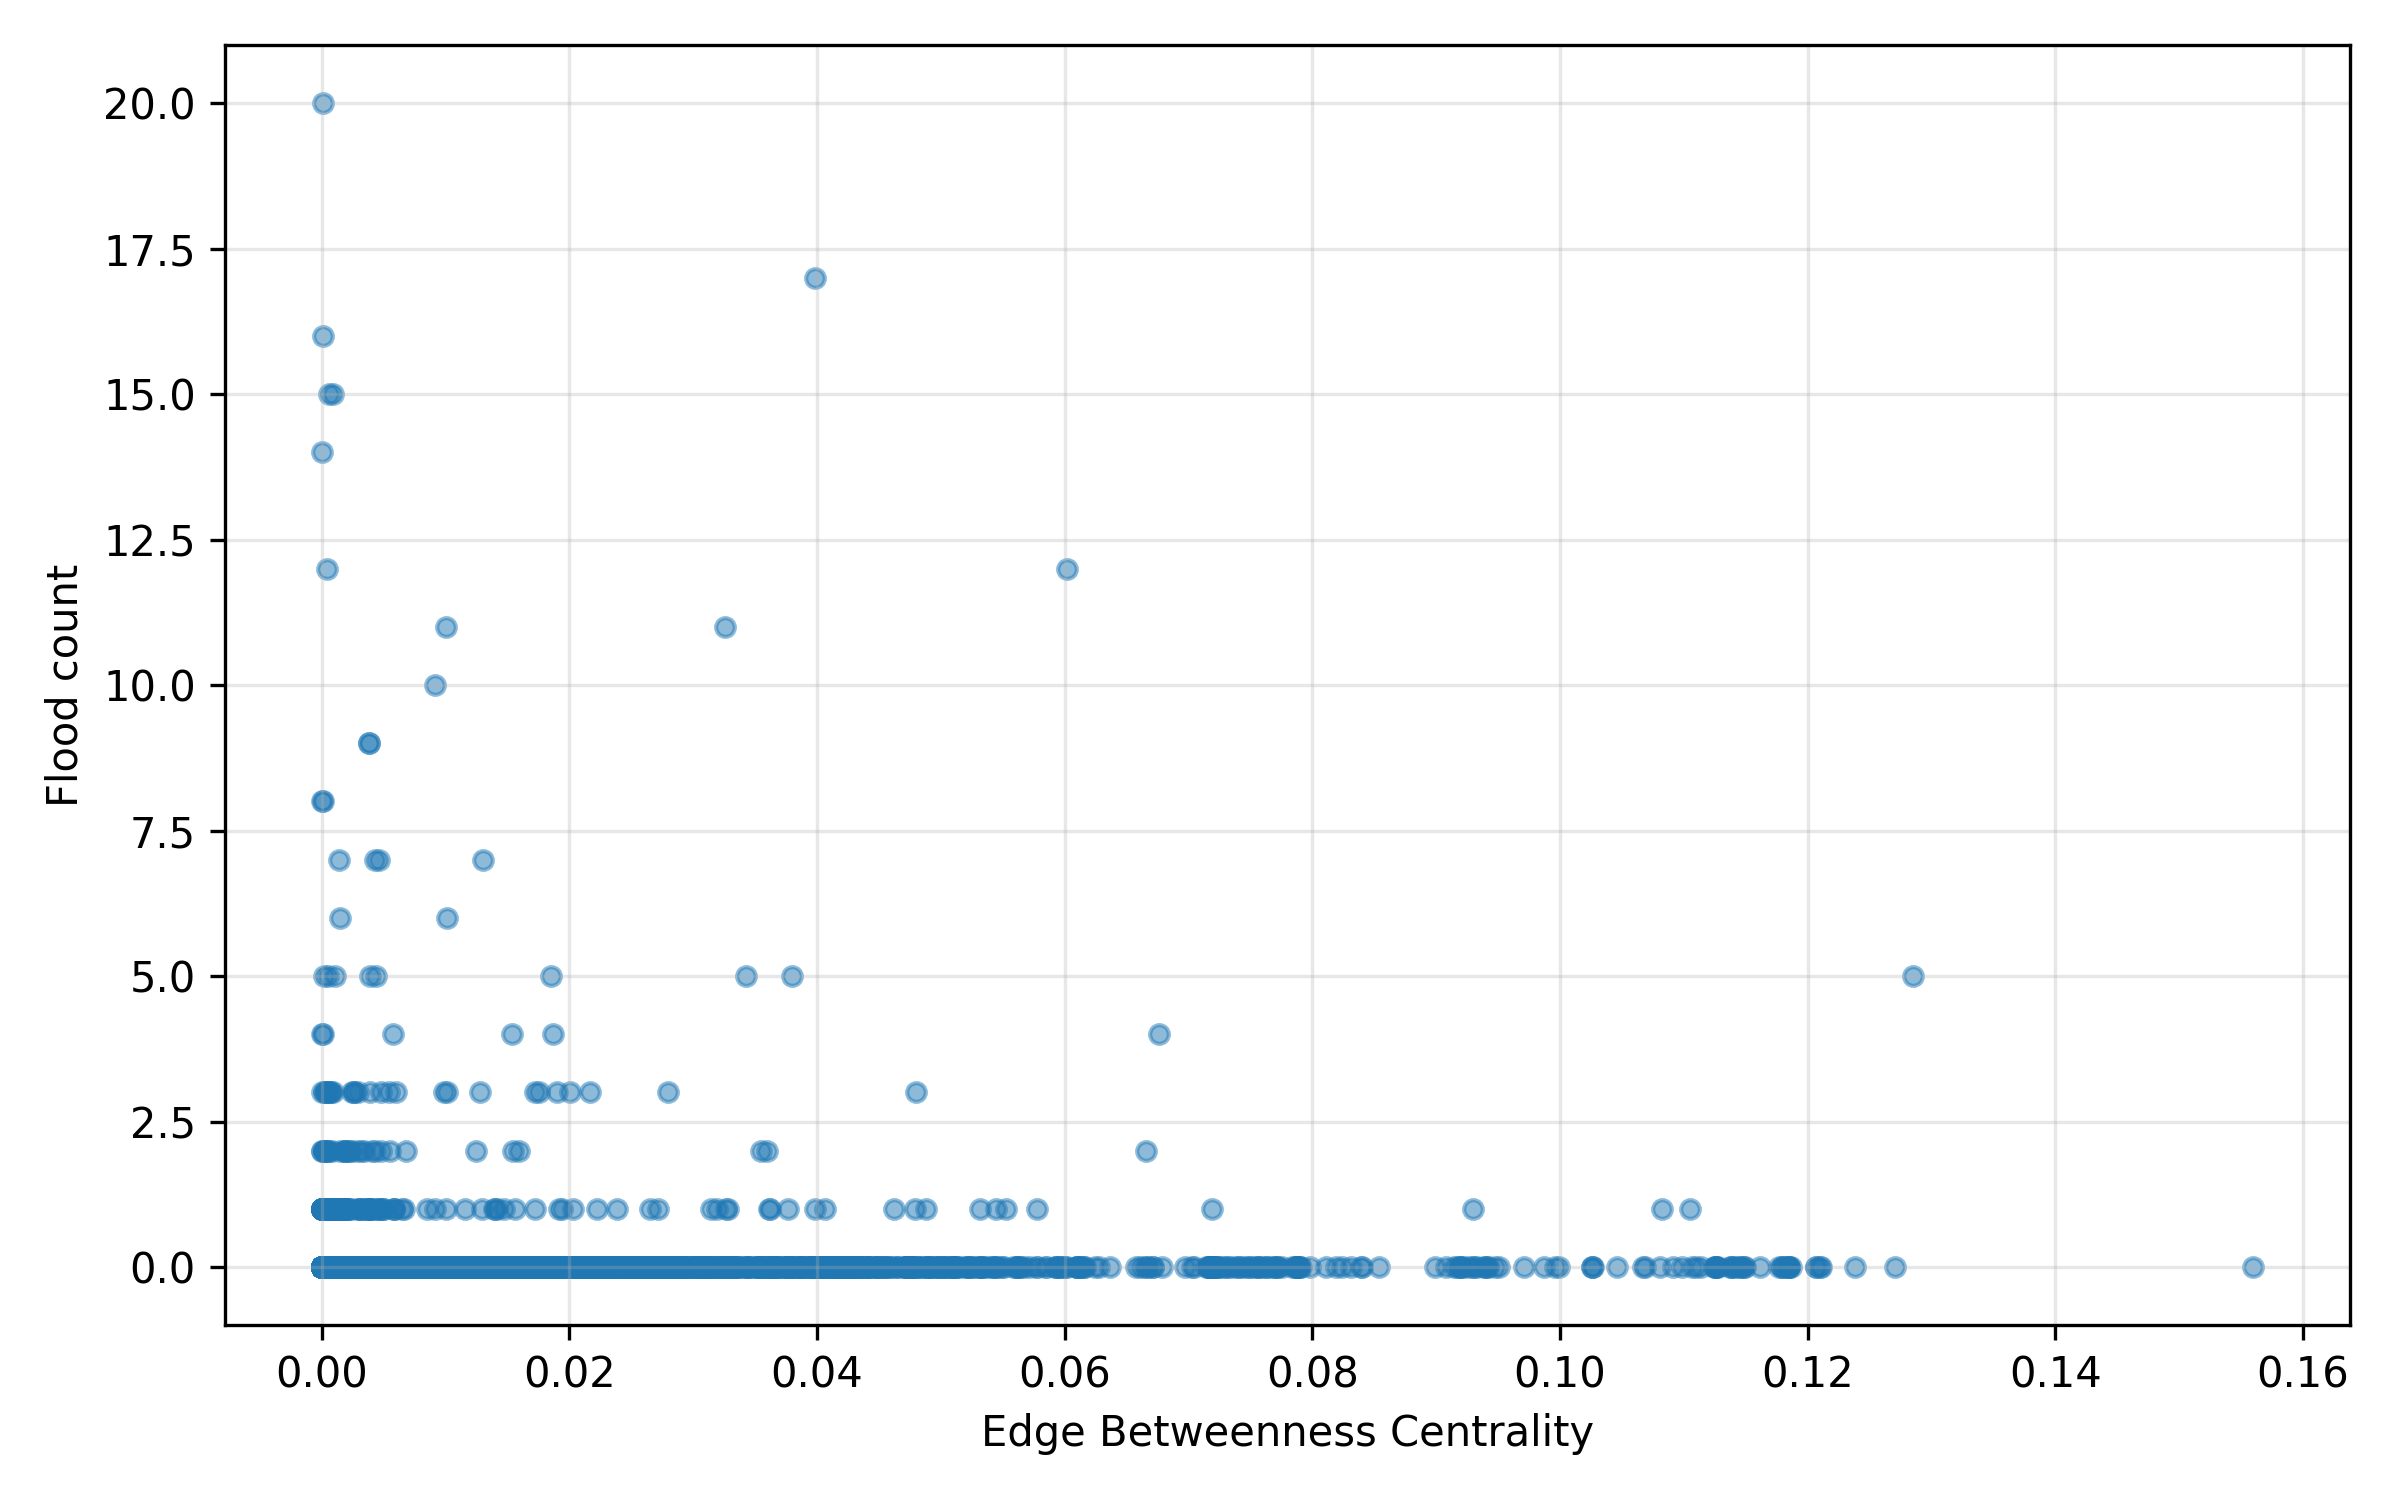
\includegraphics[width=.7\textwidth]{../plot/ebc_flood_scatter.png}
\caption{EBC and normalized flood per edge}
\label{fig:ebc-flood-scatter}
\end{figure}

Finally, Figure \ref{fig:ebc-pop-scatter} shows the relationship between the normalized population (population value per count of edges in each range of EBC) and EBC values. There is little variation in normalized population across EBC ranges, except for ranges around 0.08, which showed higher values, and around 0.16, which showed lower values.

\begin{figure}[H]
\centering
\includegraphics[width=.7\textwidth]{../plot/ebc_population_scatter.png}
\caption{EBC and normalized population per edge}
\label{fig:ebc-pop-scatter}
\end{figure}

\section{Conclusion}

In this work, it was possible to analyze the vulnerability of urban roads in São Paulo, considering the area of the city within parts of the Tamanduateí river basin, based on data of flood events, population, and network topology. Mainly, the results showed that the urban road network distribution of degree values did not follow a power-law behavior. It was observed that only a few road sections showed relatively high EBC values, with approximately half of the edges presenting values close to zero.

Some edges with EBC values between 0.06-0.07 and 0.12-0.13 presented high flood count values, normalized by the quantity of edges in each EBC range. This indicates locations where the network is more vulnerable and, therefore, more impacted by the effects of flooding events. Performing the same comparison with the population data for each edge, it was possible to observe that there is little variation in normalized population across EBC ranges, with exceptions at ranges around 0.08 (higher values) and 0.16 (lower values). This suggests that topological vulnerability does not show a clear relationship with population distribution across most of the network, and that are some more critical locations regarding exposure.

Every flood event was considered as of equal impact on the network, but the original data has an attribute that indicates the level of severity (passable or not passable flood event) that was not considered in this work. Adding new exposure data, like traffic flow, and applying graph theory methods weighted by population, flow and physical distance could improve the precision of the analysis.


%%%%%%%%%%%%%%%%%%%%%%%%%%%%%%%%%%%%%%%%%%%%%%%%%%%%%%%%%%%%%%%%%%%%%%%%
% REFS BIBLIOGRÁFICAS
% POR FAVOR, NÃO ALTERAR
%%%%%%%%%%%%%%%%%%%%%%%%%%%%%%%%%%%%%%%%%%%%%%%%%%%%%%%%%%%%%%%%%%%%%%%%
\printbibliography
%%%%%%%%%%%%%%%%%%%%%%%%%%%%%%%%%%%%%%%%%%%%%%%%%%%%%%%%%%%%%%%%%%%%%%%%

\end{document}




